%%%%%%%%%%%%%%%%%%%%%%%%%%%%%%%%%%%%%%%%%
% Beamer Presentation
% LaTeX Template
% Version 1.0 (10/11/12)
%
% This template has been downloaded from:
% http://www.LaTeXTemplates.com
%
% License:
% CC BY-NC-SA 3.0 (http://creativecommons.org/licenses/by-nc-sa/3.0/)
%
%%%%%%%%%%%%%%%%%%%%%%%%%%%%%%%%%%%%%%%%%

%----------------------------------------------------------------------------------------
% PACKAGES AND THEMES
%----------------------------------------------------------------------------------------

\documentclass[aspectratio=169]{beamer}

\mode<presentation> {

    % The Beamer class comes with a number of default slide themes
    % which change the colors and layouts of slides. Below this is a list
    % of all the themes, uncomment each in turn to see what they look like.

    %\usetheme{default}
    %\usetheme{AnnArbor}
    %\usetheme{Antibes}
    %\usetheme{Bergen}
    %\usetheme{Berkeley}
    %\usetheme{Berlin}
    %\usetheme{Boadilla}
    \usetheme{CambridgeUS}
    %\usetheme{Copenhagen}
    %\usetheme{Darmstadt}
    %\usetheme{Dresden}
    %\usetheme{Frankfurt}
    %\usetheme{Goettingen}
    %\usetheme{Hannover}
    %\usetheme{Ilmenau}
    %\usetheme{JuanLesPins}
    %\usetheme{Luebeck}
    %\usetheme{Madrid}
    %\usetheme{Malmoe}
    %\usetheme{Marburg}
    %\usetheme{Montpellier}
    %\usetheme{PaloAlto}
    %\usetheme{Pittsburgh}
    %\usetheme{Rochester}
    %\usetheme{Singapore}
    %\usetheme{Szeged}
    %\usetheme{Warsaw}

    % As well as themes, the Beamer class has a number of color themes
    % for any slide theme. Uncomment each of these in turn to see how it
    % changes the colors of your current slide theme.

    %\usecolortheme{albatross}
    %\usecolortheme{beaver}
    %\usecolortheme{beetle}
    %\usecolortheme{crane}
    %\usecolortheme{dolphin}
    %\usecolortheme{dove}
    %\usecolortheme{fly}
    %\usecolortheme{lily}
    %\usecolortheme{orchid}
    %\usecolortheme{rose}
    %\usecolortheme{seagull}
    %\usecolortheme{seahorse}
    %\usecolortheme{whale}
    %\usecolortheme{wolverine}

    %\setbeamertemplate{footline} % To remove the footer line in all slides uncomment this line
    %\setbeamertemplate{footline}[page number] % To replace the footer line in all slides with a simple slide count uncomment this line

    \setbeamertemplate{navigation symbols}{} % To remove the navigation symbols from the bottom of all slides uncomment this line
    }

    \usepackage{graphicx} % Allows including images
    \usepackage{booktabs} % Allows the use of \toprule, \midrule and \bottomrule in tables
    \usepackage{ngerman}
    \usepackage{parallel}

    %----------------------------------------------------------------------------------------
    % TITLE PAGE
    %----------------------------------------------------------------------------------------

    \title[Wärmebildkamera]{Wärmebildkamera Flir K53} % The short title appears at the bottom of every slide, the full title is only on the title page

    \author{Alex Leuck \& Samuel Scherer} % Your name
    \institute[] % Your institution as it will appear on the bottom of every slide, may be shorthand to save space
    {
    \normalsize Feuerwehr Heidelberg \\ % Your institution for the title page
    \scriptsize{Abteilung Neuenheim} \\
    \medskip
    \textit{alexander.leuck@feuerwehr-neuenheim.de \\ samuel.scherer@feuerwehr-neuenheim.de} % Your email address
    }
    \date{\today} % Date, can be changed to a custom date

    \begin{document}

    \begin{frame}
    \titlepage % Print the title page as the first slide
    \end{frame}

    \begin{frame}
    \frametitle{Inhalt} % Table of contents slide, comment this block out to remove it
    \tableofcontents % Throughout your presentation, if you choose to use \section{} and \subsection{} commands, these will automatically be printed on this slide as an overview of your presentation
    \end{frame}

    %----------------------------------------------------------------------------------------
    % PRESENTATION SLIDES
    %----------------------------------------------------------------------------------------

    %------------------------------------------------
    \section{Warum brauchen wir eine Wärmebildkamera?} % Sections can be created in order to organize your presentation into discrete blocks, all sections and subsections are automatically printed in the table of contents as an overview of the talk
    %------------------------------------------------

    %\subsection{Subsection Example} % A subsection can be created just before a set of slides with a common theme to further break down your presentation into chunks

    \begin{frame}
    \frametitle{Strahlungsintensität}
    \centering{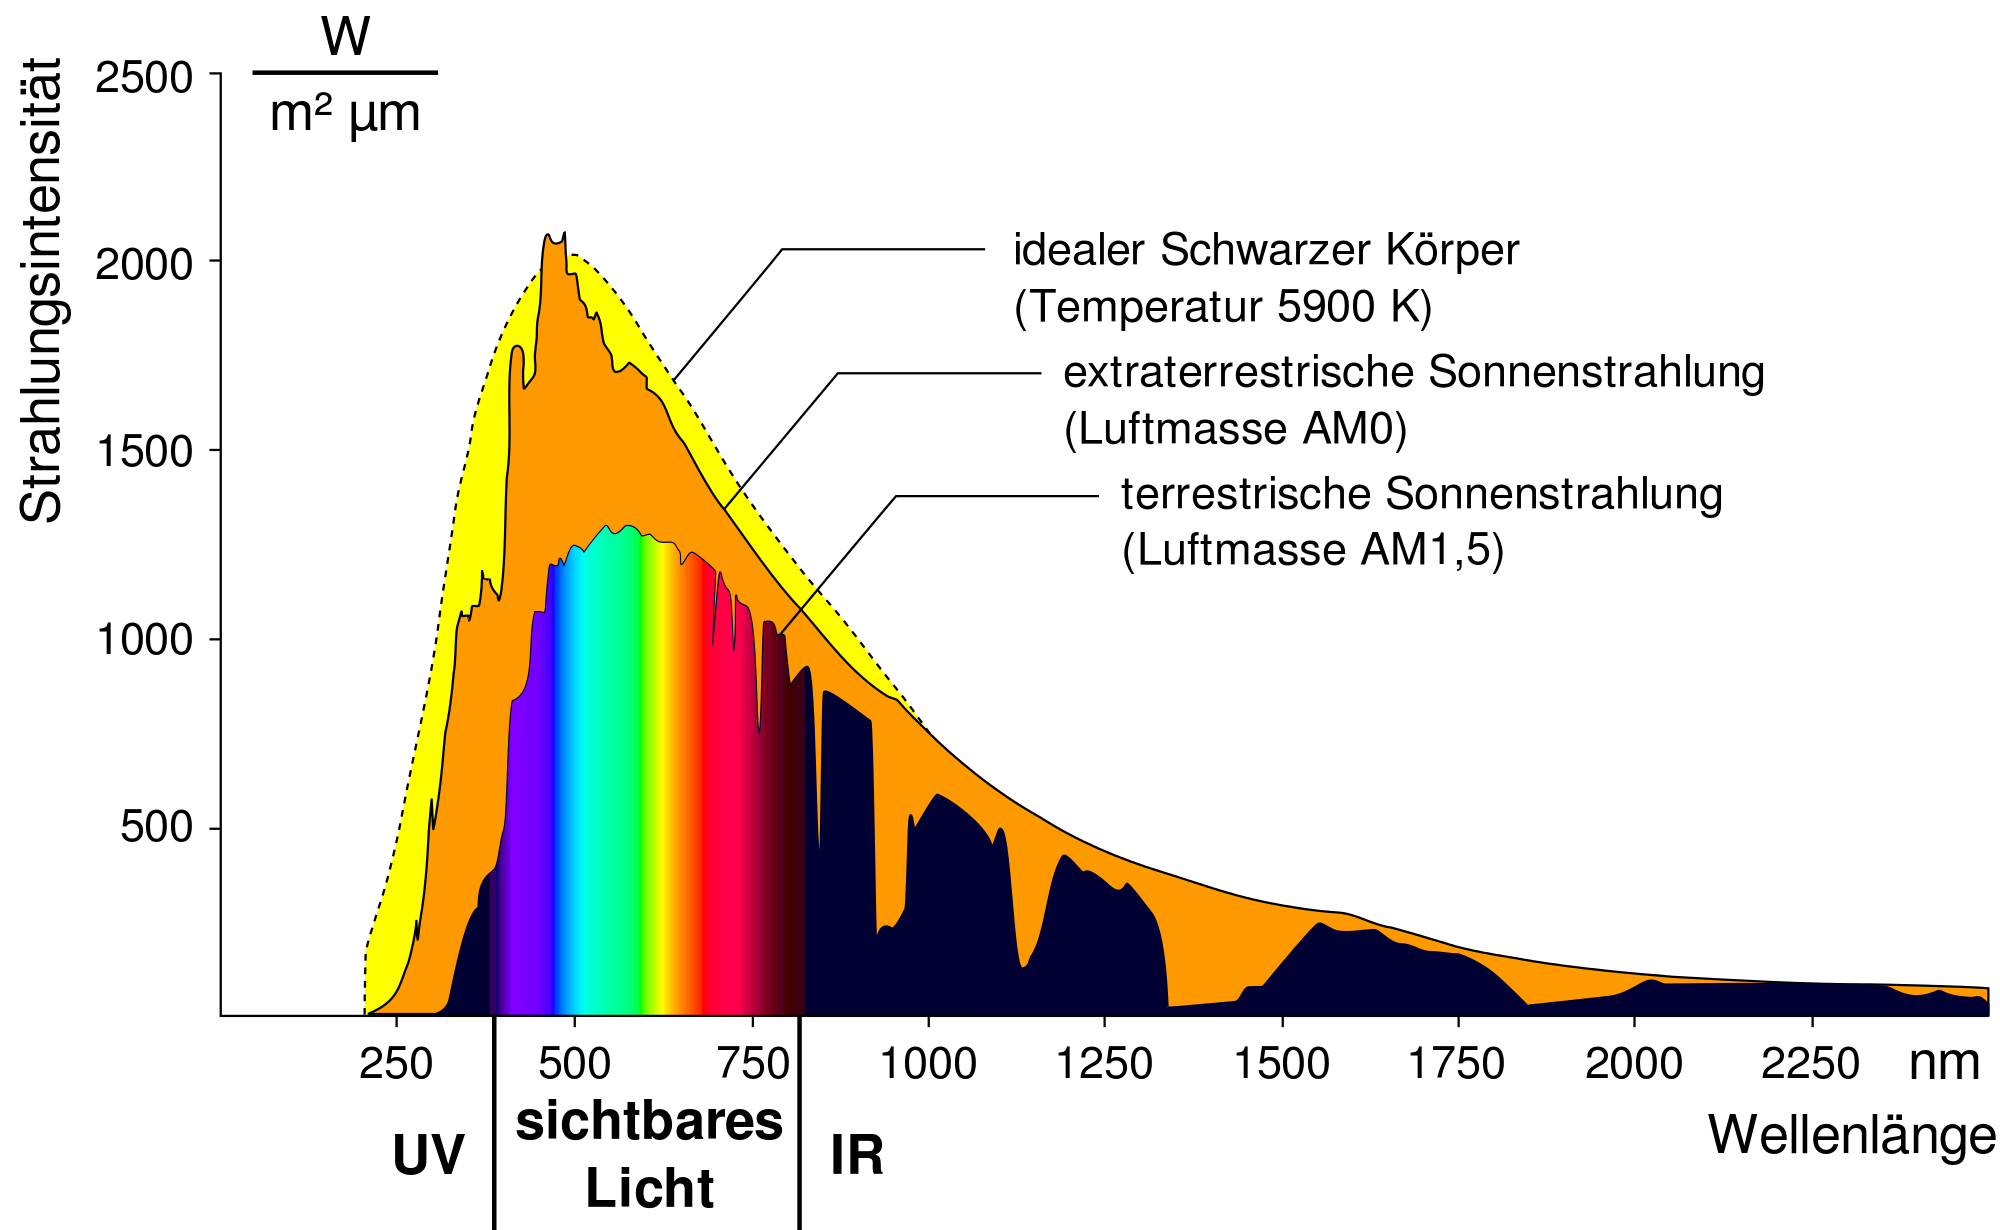
\includegraphics[width=0.7\textwidth, keepaspectratio]{strahlung}}
    \end{frame}

    %------------------------------------------------

    \section{Bedienung der Flir K53}
    \begin{frame}
    \frametitle{Bedienung der Flir K53}
    \centering{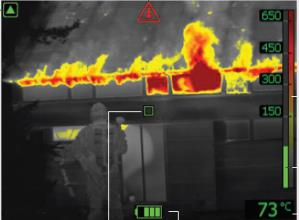
\includegraphics[width=0.6\textwidth, keepaspectratio]{display}}
    \end{frame}

    %------------------------------------------------
    \section{Einsatzmöglichkeiten}
    \begin{frame}[t]
    \frametitle{Einsatzmöglichkeiten}
    \begin{itemize}
    \item Wann nehmen wir die WBK mit?
    \begin{itemize}
    \item<2-> Nach SER: AT-Führer nimmt sie immer mit.
        \item<3-> wir lassen sie auf dem LF, wenn offensichtlich
            \end{itemize}
            \end{itemize}
            \end{frame}
            \begin{frame}
            \centering{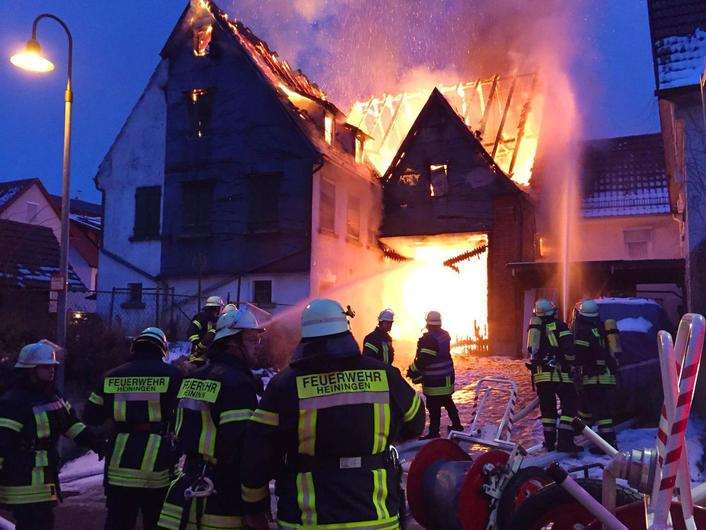
\includegraphics[width=0.7\textwidth, keepaspectratio]{keinewbk}}
            \end{frame}

            \begin{frame}[t]
            \frametitle{Einsatzmöglichkeiten}
            \begin{itemize}
            \item Wann nehmen wir die WBK mit?
            \begin{itemize}
            \item Nach SER: AT-Führer nimmt sie immer mit.
            \item lasst sie da, wenn offensichtlich
            \end{itemize}
            \item<2-> Nutzung im Einsatz:
                \begin{itemize}
                \item<3-> Personensuche (Brand/VU/Wasserrettung)
                    \item<4-> Suche nach Brandherd und Glutnestern
                        \item<5-> Einschätzen der Temperatur von z.B. Gasflaschen/Türen
                            \item<6-> Füllstände von Fässern und Kesselwaggons
                                \end{itemize}
                                \item[]<3-> 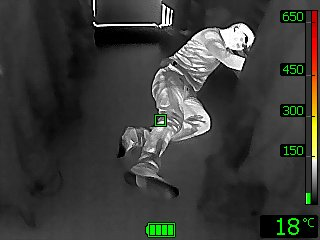
\includegraphics[width=0.3\textwidth, keepaspectratio]{wuerfelblick_raw/boden} 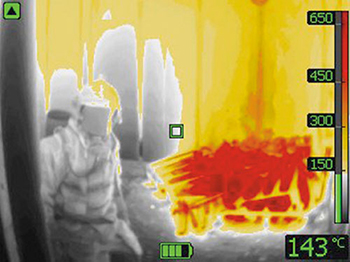
\includegraphics[width=0.3\textwidth, keepaspectratio]{feuer}<4->
                                        \end{itemize}
                                        \end{frame}

                                        %------------------------------------------------

                                        \section{Einsatzgrundsätze/-taktik}
                                        \begin{frame}
                                        \frametitle{Einsatzgrundsätze/-taktik}
                                        \begin{columns}
                                        \begin{column}{0.3\textwidth}
                                        \begin{enumerate}
                                        \item<2-> Gehen
                                        \item<3-> Schauen
                                        \item<5-> Handeln
                                        \item<6-> Kontrollieren
                                        \item<7-> Korrigieren
                                        \end{enumerate}
                                        \end{column}
                                        \begin{column}{0.7\textwidth}
                                        \begin{center}
                                        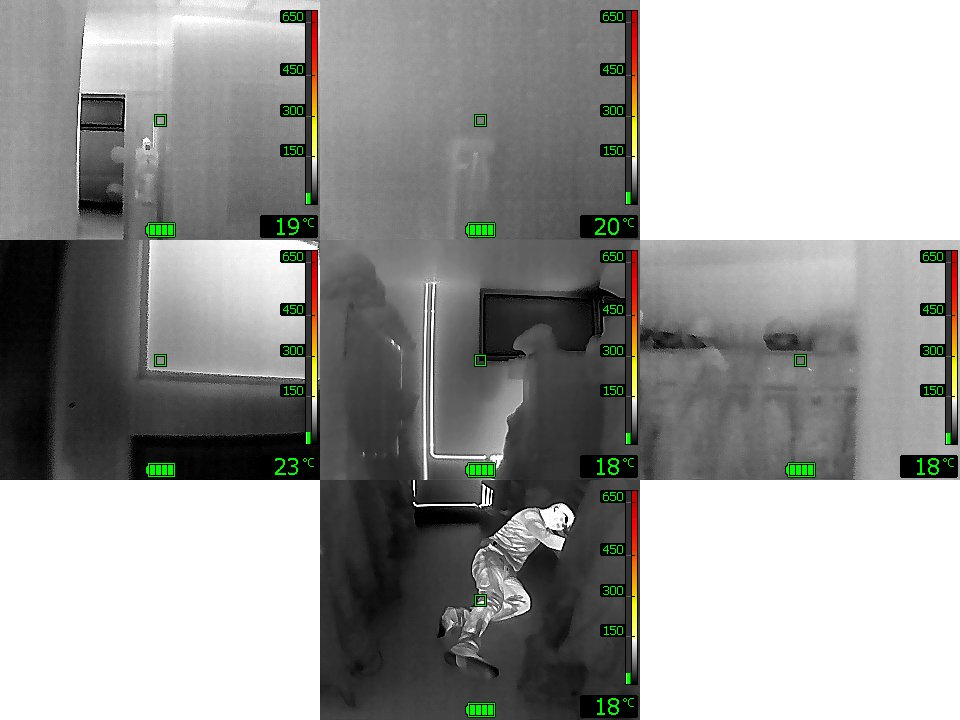
\includegraphics[width=0.7\textwidth, keepaspectratio]{wuerfelblick}<4->
                                        \end{center}
                                        \end{column}
                                        \end{columns}
                                        \end{frame}

                                        %------------------------------------------------
                                        \begin{frame}
                                        \begin{center}
                                        \color{red}
                                        \huge{Wichtig:} \\
                                        \normalsize
                                        \pause Die WBK ist keine Rückzugsicherung! \\
                                        \pause Nicht während der Nutzung der WBK gehen! \\
                                        \pause Auf Fehlerquellen achten! \\
                                        
                                        \end{center}
                                        \end{frame}

                                        \section{Praktische Übungen}
                                        \begin{frame}
                                        \Huge{\centerline{Praktische Übungen}}
                                        \end{frame}

                                        %----------------------------------------------------------------------------------------

                                        \end{document}
